\chapter{Deep Learning}
	\label{chap:deep-learning}
		In questo capitolo sarà introdotto il deep learning, verranno descritte architetture di reti neurali semplici fino ad arrivare ad alcune più complesse utilizzate in questo lavoro.
		
		\section{Introduzione}
		Il deep learning è una branca del machine learning che si basa sull'apprendimento della rappresentazione dei dati. A differenza dei tipici approcci in cui si scrive un algoritmo per svolgere un'attività specifica, si realizzano invece degli algoritmi in grado di imparare a mappare dati tra domini differenti.
		Questa disciplina prende forte ispirazione dall'organizazione del cervello che, attraverso diverse trasformazioni e rappresentazioni, riesce ad imparare a processare le informazioni.
		
		\section{Percettrone}
		Un percettrone è l'architettura neurale minima, introdotta nel 1958 da Rosenblatt\cite{perceptron}, ed è ispirata al funzionamento del neurone, unità minima del cervello umano. Esattamente come un neurone esso infatti riceve dei segnali di ingresso e applica una somma pesata come segue:
		\begin{equation}
			y = w_0 + \sum_{i=1}^n x_i w_i
		\end{equation}
		L'output $y$ viene poi passato ad una funzione di attivazione che deciderà se il percettrone deve attivarsi o meno.
		\usetikzlibrary{positioning}
\tikzset{basic/.style={draw,fill=blue!20,text width=1.2em,text badly centered}}
\tikzset{input/.style={basic,circle}}
\tikzset{weights/.style={basic,rectangle}}
\tikzset{functions/.style={basic,circle,fill=blue!10}}
\begin{figure}%[h]
	\centering
	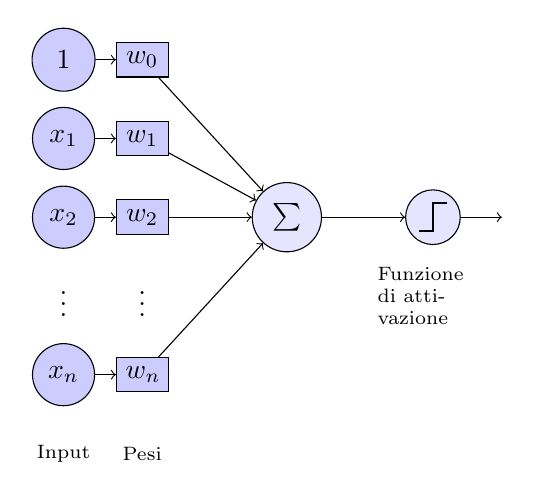
\begin{tikzpicture}
		\node[functions] (center) {};
		\node[below of=center,font=\scriptsize,text width=4em] {Funzione di attivazione};
		\draw[thick] (0.5em,0.5em) -- (0,0.5em) -- (0,-0.5em) -- (-0.5em,-0.5em);
		\node[right of=center] (right) {};
		\path[draw,->] (center) -- (right);
		\node[functions,left=3em of center] (left) {$\sum$};
		\path[draw,->] (left) -- (center);
		\node[weights,left=3em of left] (2) {$w_2$} -- (2) node[input,left of=2] (l2) {$x_2$};
		\path[draw,->] (l2) -- (2);
		\path[draw,->] (2) -- (left);
		\node[below of=2] (dots) {$\vdots$} -- (dots) node[left of=dots] (ldots) {$\vdots$};
		\node[weights,below of=dots] (n) {$w_n$} -- (n) node[input,left of=n] (ln) {$x_n$};
		\path[draw,->] (ln) -- (n);
		\path[draw,->] (n) -- (left);
		\node[weights,above of=2] (1) {$w_1$} -- (1) node[input,left of=1] (l1) {$x_1$};
		\path[draw,->] (l1) -- (1);
		\path[draw,->] (1) -- (left);
		\node[weights,above of=1] (0) {$w_0$} -- (0) node[input,left of=0] (l0) {$1$};
		\path[draw,->] (l0) -- (0);
		\path[draw,->] (0) -- (left);
		\node[below of=ln,font=\scriptsize] {Input};
		\node[below of=n,font=\scriptsize] {Pesi};
	\end{tikzpicture}
	\caption{Un percettrone con una funzione di attivazione sull'output.}
\end{figure}
		
		\section{Funzione di attivazione}
		Una funzione di attivazione è una trasformazione non lineare applicata all'output di un percettrone al fine di mapparlo in un range di valori differente.
		Si descrivono a seguire alcune delle più note funzioni di attivazione.
		\paragraph{Sigmoid}
		La funzione Sigmoid (Fig. \ref{fig:sigmoid}) è stata storicamente la più usata tra le funzioni di attivazione. Essa offre il vantaggio di mappare i valori nell'intervallo (0,1).
		\[ \sigma(z) = \frac{1} {1 + e^{-z}} \]
		\begin{figure}%[h]
			\centering
			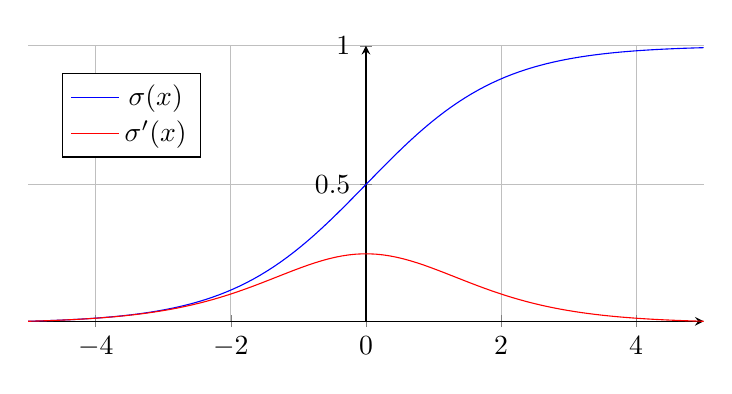
\begin{tikzpicture}[
				declare function={sigma(\x)=1/(1+exp(-\x));
				sigmap(\x)=sigma(\x)*(1-sigma(\x));}]
				\begin{axis}%
					[
					width=4in,
					height=2in,
					grid=major, 
					xmin=-5,
					xmax=5,
					axis x line=bottom,
					ytick={0,.5,1},
					ymax=1,
					axis y line=middle,
					samples=100,
					domain=-5:5,
					legend style={at={(0.05,0.9)},anchor=north west}
					]
					\addplot[blue,mark=none] (x,{sigma(x)});
					\addplot[red,mark=none] (x,{sigmap(x)});
					\legend{$\sigma(x)$,$\sigma'(x)$}
				\end{axis}
			\end{tikzpicture}
			\caption{Grafico della funzione Sigmoid.}
			\label{fig:sigmoid}
		\end{figure}
		
		\paragraph{Tanh}
		La funzione Tanh (Fig. \ref{fig:tanh}) è anch'essa sigmoidea. La principale differenza che la distingue da Sigmoid è che il suo dominio di output è in (-1,1)  che la rende particolarmente adatta nei problemi di classificazione con due classi.
		\[ tanh(x) = \frac{e^x - e^{-x}}{e^x + e^{-x}} = \frac{1 - e^{-2x}}{1 + e^{-2x}} \]
		\begin{figure}%[h]
		\centering
		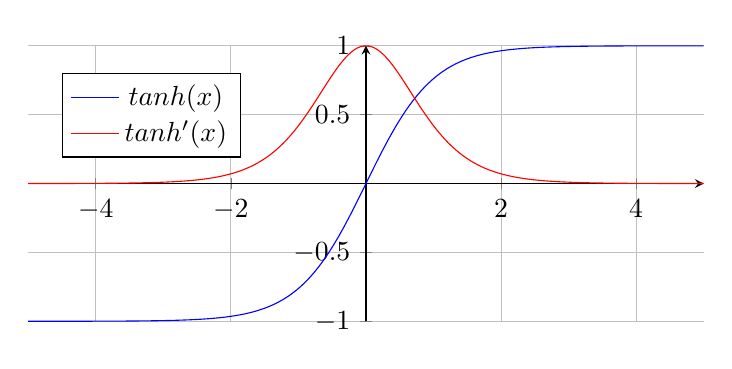
\begin{tikzpicture}
			\begin{axis}%
				[
				width=4in,
				height=2in,
				grid=major,
				xmin=-5,
				xmax=5,
				axis x line=center,
				ymax= 1,
				ymin= -1,
				axis y line=middle,
				samples=500,
				domain=-5:5,
				legend style={at={(0.05,0.9)},anchor=north west}
				]
				\addplot[blue,mark=none] (x,{tanh(x)});
				\addplot[red,mark=none] (x,{1-(tanh(x)*tanh(x))});
				\legend{$tanh(x)$,$tanh'(x)$}
			\end{axis}
		\end{tikzpicture}
		\caption{Grafico della funzione Tanh.}
		\label{fig:tanh}
		\end{figure}
		
		\paragraph{ReLU}
		La funzione ReLU (Fig. \ref{fig:relu}) è il nuovo standard per molti tipi di reti neurali in quanto permette di abbassare notevolmente il costo computazionale dell'addestramento del modello. Essa è una funzione lineare definita a tratti, che mappa in zero tutti i numeri negativi e gli altri nell'input stesso\cite{ReLU}.
		\[ ReLU(z) = max(0, z) \]
		\begin{figure}%[h]
			\centering
			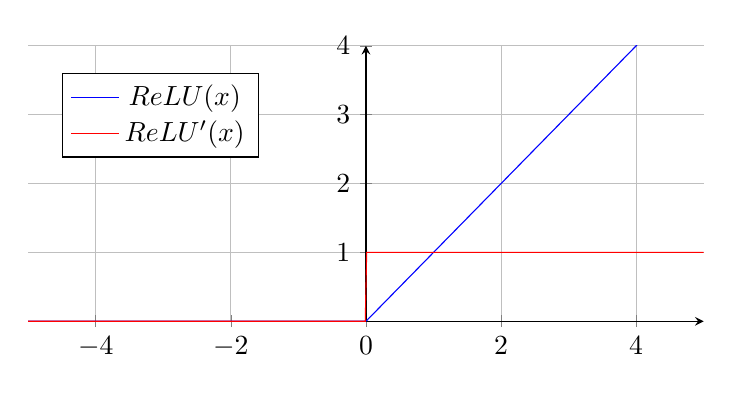
\begin{tikzpicture}
				\begin{axis}%
					[
					width=4in,
					height=2in,
					grid=major, 
					xmin=-5,
					xmax=5,
					axis x line=bottom,
					ymax= 4,
					axis y line=middle,
					samples=500,
					domain=-5:5,
					legend style={at={(0.05,0.9)},anchor=north west}
					]
					\addplot[blue,mark=none] (x,{max(0,x)});
					\addplot[red,mark=none] (x,{(x>0)});
					\legend{$ReLU(x)$,$ReLU'(x)$}
				\end{axis}
			\end{tikzpicture}
			\caption{Grafico della funzione ReLU.}
			\label{fig:relu}
		\end{figure}
		
		\section{Rete neurale artificiale}
		I percettroni sono solitamente organizzati in livelli, che possono avere strutture diverse per effettuare trasformazioni differenti. Una rete neurale artificiale (ANN) è formata da più livelli interconnessi e organizzati come segue:
		\begin{itemize}
			\item \textbf{Livello di input}: ottiene i dati iniziali per la rete neurale.
			\item \textbf{Livelli nascosti}: livelli intermedi che svolgono la computazione.
			\item \textbf{Livello di output}: produce il risultato finale.
		\end{itemize}
		Il tipo di ANN più semplice è una Multilayer Perceptron (MLP), un'architettura fully connected e feedforward, ovvero in cui ogni nodo in uscita è connesso ad ogni altro nodo del livello successivo (Fig. \ref{fig:mlp}).
		% !TeX encoding = UTF-8
% !TeX program = pdflatex
% !TeX spellcheck = it_IT
\usetikzlibrary{positioning}
\tikzset{%
	every neuron/.style={
		circle,
		draw,
		minimum size=1cm
	},
	neuron missing/.style={
		draw=none, 
		scale=2,
		text height=0.333cm,
		execute at begin node=\color{black}$\vdots$
	},
}
\begin{figure}[h]
\centering
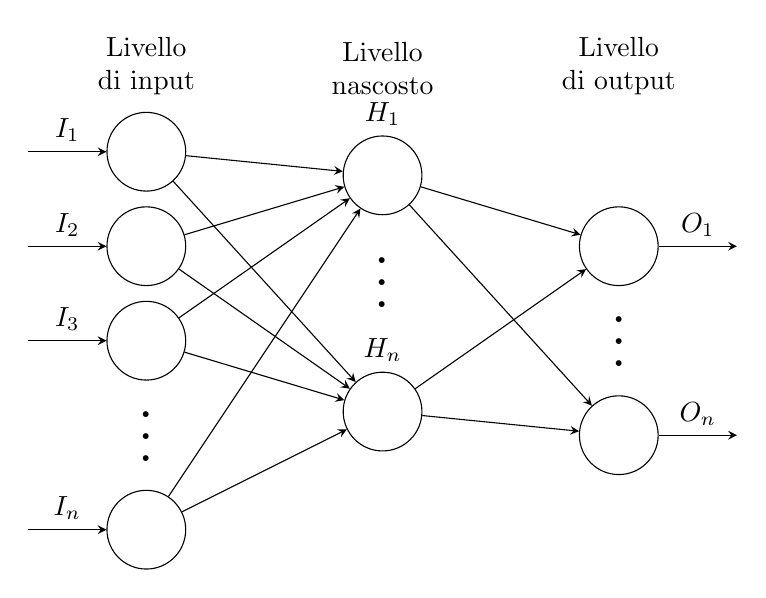
\begin{tikzpicture}[x=1.5cm, y=1.2cm, >=stealth]
	
	\foreach \m/\l [count=\y] in {1,2,3,missing,4}
	\node [every neuron/.try, neuron \m/.try] (input-\m) at (0,2.5-\y) {};
	
	\node [every neuron/.try, neuron 1/.try ] (hidden-1) at (2, 1.25) {};
	\node [every neuron/.try, neuron missing/.try ] (hidden-missing) at (2, 0.1*1.25) {};
	\node [every neuron/.try, neuron 1/.try ] (hidden-2) at (2, -1*1.25) {};	
	
	\foreach \m [count=\y] in {1,missing,2}
	\node [every neuron/.try, neuron \m/.try ] (output-\m) at (4,1.5-\y) {};
	
	\foreach \l [count=\i] in {1,2,3,n}
	\draw [<-] (input-\i) -- ++(-1,0)
	node [above, midway] {$I_\l$};
	
	\foreach \l [count=\i] in {1,n}
	\node [above] at (hidden-\i.north) {$H_\l$};
	
	\foreach \l [count=\i] in {1,n}
	\draw [->] (output-\i) -- ++(1,0)
	node [above, midway] {$O_\l$};
	
	\foreach \i in {1,...,4}
	\foreach \j in {1,...,2}
	\draw [->] (input-\i) -- (hidden-\j);
	
	\foreach \i in {1,...,2}
	\foreach \j in {1,...,2}
	\draw [->] (hidden-\i) -- (output-\j);
	
	\foreach \l [count=\x from 0] in {di input, nascosto, di output}
	\node [align=center, above] at (\x*2,2) {Livello \\ \l};
	
\end{tikzpicture}
\caption{Grafo rappresentante una MLP.}
\label{fig:mlp}
\end{figure}
		
		\section{Algoritmi di apprendimento}
		Gli algoritmi di machine learning si possono suddividere in tre categorie in base alle modalità di svolgimento della fase di addestramento\cite{deep-learning-book}:
		\begin{itemize}
			\item \textbf{Supervised Learning}: paradigma applicabile laddove sia presente un dataset con elementi che abbiano un'etichetta applicata o che abbiano un corrispondente elemento obiettivo, utile ai fini di classificazione o regressione.
			\item \textbf{Unsupervised Learning}: paradigma applicabile laddove sia utile imparare proprietà sulla struttura dei dati, come per la generazione o la riduzione del rumore da essi.
			\item \textbf{Semi-supervised Learning}: sfrutta sia tecniche del supervised learning, sia dell'unsupervised learning. Nello specifico si sfrutta la conoscenza fornita dai dati etichettati per classificare anche i restanti. Questa tecnica agevola la costruzione del dataset in quanto si possono usare più dati ma richiede comunque una prevalenza di dati etichettati.
		\end{itemize}
		
		\section{Reti neurali avanzate}
		In questa sezione vengono descritte le principali reti neurali avanzate utilizzate in questo lavoro.
		
		\subsection{CNN}
		Una CNN (Convolutional Neural Network) è una tipologia di rete neurale artificiale comunemente utilizzata nella classificazione di immagini (Fig. \ref{fig:cnn})\cite{cnn}. La rete è composta in genere da tre tipi di livelli:
		\begin{itemize}
			\item \textbf{Livelli convoluzionali}: applicano dei filtri alle immagini al fine di estrarre feature da esse.
			\item \textbf{Livelli di pooling}: riducono lo spazio di rappresentazione raccogliento output vicini basandosi su calcoli statistici come media o massimo.
			\item \textbf{Livelli fully connected}: connettono tutti i nodi tra loro in modo da poter permettere la classificazione basandosi sulle feautre estratte. 
		\end{itemize}
		\begin{figure}[h]
			\centering
			\includegraphics[width=0.7\linewidth]{figures/CNN}
			\caption{Convolutional Neural Network per la classificazione di immagini. Fonte https://it.mathworks.com/discovery/convolutional-neural-network-matlab.html.}
			\label{fig:cnn}
		\end{figure}
		
		\subsection{GAN}
			Una GAN (Generative Adversarial Network) è una classe di algoritmi di deep learning proposta nel 2014 da Goodfellow\cite{Goodfellow}. Consiste in due reti neurali che competono in un gioco a somma zero (\ref{eq:gan}), addestrando due modelli allo stesso tempo: un modello generativo (G) e un modello discriminatore (D).
			La rete generativa produrrà immagini che verranno passate in input alla rete discriminatore mentre quest'ultima si occuperà di classificarle come reali o generate (Fig. \ref{fig:gans}).
			\begin{equation}
				\min_G\max_D{V(D, G)} = \min_G\max_D \left[\; \mathbb{E}_{x \sim p_{data}}[log \; D(x)] + \; \mathbb{E}_{z \sim p_{z}}[log \; (1 - D(G(z)))] \right]
				\label{eq:gan}
			\end{equation}
			
			Il discriminatore è un classificatore che impara a distinguere dati reali da quelli creati dal generatore, questo sarà addestrato usando dati reali e l'output del generatore, e verrà penalizzato in caso classifichi scorrettamente i dati e aggiornando i suoi pesi attraverso backpropagation.
			
			Il generatore è una rete che impara a generare immagini false che sembrino realistiche, questo sarà addestrato usando dati casuali e il suo output verrà collegato al discriminatore, e verrà penalizzato in caso esso rilevi l'immagine generata come falsa.
			
			\begin{figure}[h]
				\centering
				\includegraphics[width=0.7\linewidth]{figures/gans}
				\caption{GAN che genera dipinti in stile Monet.}
				\label{fig:gans}
			\end{figure}
		
		\subsection{CycleGAN}
			La \textit{image-to-image translation} è una classe di problemi nelle quali l'obiettivo è riuscire a imparare a mappare input e output di coppie di immagini. Tuttavia avere a disposizione questi dati paralleli non è sempre possibile. Basti pensare ad un convertitore di foto a dipinti, bisognerebbe dunque avere una serie di foto e dipinti corrispondenti e abbinate.
			
			Nella image-to-image translation la GAN come input, anziché rumore casuale, prende un'immagine di un certo dominio $X$ e cercherà di mapparla in un'immagine generata che abbia proprietà simili al dominio $Y$ (immagini date di rifermento al discriminatore).
			Al fine di costruire un framework che permetta di lavorare con dati non paralleli, semplificando quindi la collezione del dataset, è stata progettata la CycleGAN\cite{CycleGAN2017}.
			
			Una CycleGAN è composta da 2 GAN, una per convertire dal dominio $X$ al dominio $Y$ e una per l'inverso, e dunque da 2 generatori e 2 discriminatori.
			Nella fase di training abbiamo due cicli che si alternano: un ciclo forward e uno backward. 
			Nel ciclo forward (Fig. \ref{fig:cyclegan-forward}) viene selezionata un'immagine dal dominio $X$ e viene trasformata dal primo generatore ($G_{XY}$) in un'immagine del dominio $Y$. Questa viene testata dal discriminatore che dovrà capire se sia reale o generata. La stessa immagine viene anche trasformata nuovamente dal secondo generatore ($G_{YX}$) in un'immagine del dominio $X$ per poi essere confrontata impiegando una funzione di \textit{Cycle Consistency Loss} con l'immagine originale.

			\begin{figure}%[h]
				\centering
				\includegraphics[width=1\linewidth]{figures/cyclegan-A2B}
				\caption{Ciclo forward della CycleGAN che trasforma foto in dipinti di Monet.}
				\label{fig:cyclegan-forward}
			\end{figure}
			
			Nel ciclo backward avviene la stessa operazione del ciclo forward ma partendo dal dominio $Y$ e usando gli opportuni generatori e discrimantori come illustrato in Fig. \ref{fig:cyclegan-backward}.
			\begin{figure}%[h]
			\centering
			\includegraphics[width=1\linewidth]{figures/cyclegan-B2A}
			\caption{Ciclo backward della CycleGAN che trasforma foto in dipinti di Monet.}
			\label{fig:cyclegan-backward}
			\end{figure}
	
		\subsection{MelGAN}
		Elaborare segnali audio è un processo complesso che richiede spesso il passaggio a rappresentazioni intermedie che possono portare artefatti e comprometterne i risultati.
		Nel 2019 viene proposto da Kumar un vocoder neurale per spettrogrammi mel basato su reti generative avversarie: MelGAN\cite{melgan}.
		L'architettura è una fully convolutional network che prende in input spettrogrammi mel e fornisce come output l'audio corrispondente.
		
		\subsection{CycleGAN-VCs}
			Di seguito vengono descritte le architetture delle CycleGAN-VCs per poter vedere quali sono i passi che hanno portato ad ottenere la MaskCycleGAN-VC, ovvero la rete impiegata in questo lavoro.
			
			\paragraph{CycleGAN-VC}
			Nel 2017 Kaneko e Kameoka propongono un metodo per la voice conversion che permette di imparare a mappare una voce source in una target senza bisogno di dati paralleli. Il metodo, chiamato CycleGAN-VC, si basa sull'architettura di una CycleGAN a cui vengono applicate due modifiche: l'impiego di gated CNN e l'impiego di una identity-mapping loss (Fig. \ref{fig:cyclegan-vc})\cite{CycleGAN-VC}.
			
			L'introduzione di gated CNN all'interno della rete permette di conservare la struttura gerarchica della voce mantenendo un costo computazionale piuttosto basso mentre l'impiego di una funzione di identità (\ref{eq:identity}) ha lo scopo di mantenere il contenuto linguistico intatto.
			\begin{equation}
				\mathcal{L}_{id}(G_{XY}, G_{YX}) = \mathbb{E}_{y \sim P_{Data}(y)}[||G_{XY}(y) - y||_1] \\
				+ \mathbb{E}_{x \sim P_{Data}(x)}[||G_{YX}(x) - x||_1]
			\label{eq:identity}
			\end{equation}
			
			\begin{figure}[h]
				\centering
				\includegraphics[width=1\linewidth]{figures/CycleGAN-VC}
				\caption{Architettura di CycleGAN-VC. Fonte \cite{CycleGAN-VC}.}
				\label{fig:cyclegan-vc}
			\end{figure}
		
			Il modello utilizza coefficienti mel cepstrum, frequenza fondamentale logaritmica e aperiodicità come feature per la conversione.
			I risultati ottenuti sono di particolare interesse in quanto simili a procedure con impiego di dati paralleli senza necessitare di ulteriori dati o dell'allineamento temporale di questi.
		
			\paragraph{CycleGAN-VC2}
			Successivamente, nel 2019 viene proposta una versione migliorata, chiamata CycleGAN-VC2 (Fig. \ref{fig:cyclegan-vc2}), che incorpora tre principali cambiamenti: introduzione di una seconda adversarial loss (\ref{eq:second-loss}), generatore migliorato (2-1-2D CNN) e discriminatore migliorato (PatchGAN)\cite{CycleGAN-VC2}. 
			\begin{equation}
				\mathcal{L}_{adv2}^{X \rightarrow Y \rightarrow X} = \mathbb{E}_{x \sim P_X}[log D'_X(x)] + \mathbb{E}_{x \sim P_X}[log(1-D'_X(G_{YX}(G_{XY}(x))))]
				\label{eq:second-loss}
			\end{equation}
			
			\begin{figure}[h]
				\centering
				\includegraphics[width=1\linewidth]{figures/CycleGAN-VC2}
				\caption{Architettura di CycleGAN-VC2. Fonte \cite{CycleGAN-VC2}.}
				\label{fig:cyclegan-vc2}
			\end{figure}
			
			\paragraph{CycleGAN-VC3}
			Gli ottimi risultati ottenuti dalle CycleGAN-VCs hanno portato all'impiego di queste come metodi di benchmark per altri studi. Questo però ha evidenziato la necessità di confrontare i risultati sotto forma di spettrogrammi mel. Tuttavia impiegando spettrogrammi mel, al posto di coefficienti mel cepstrum, direttamente come input di queste reti, si producono risultati scarsi dovuti alla compromissione della struttura temporale del segnale.
			
			Al fine di ovviare a questo problema viene proposta CycleGAN-VC3 (Fig. \ref{fig:cyclegan-vc3}) che incorpora una normalizzazione adattiva sul dominio tempo-frequenza (TFAN)\cite{CycleGAN-VC3}.
			\begin{figure}[h]
				\centering
				\includegraphics[width=0.8\linewidth]{figures/CycleGAN-VC3}
				\caption{Comparazione di CycleGAN-VC3 rispetto a CycleGAN-VC2. In CycleGAN-VC3 viene incorporato TFAN nel generatore di CycleGAN-VC2. In particolare viene rimpiazzato nel blocco 1D$\rightarrow$2D e nel blocco Upsample. Fonte \cite{CycleGAN-VC3}.}
				\label{fig:cyclegan-vc3}
			\end{figure}
		
			\paragraph{MaskCycleGAN-VC}
			La MaskCycleGAN-VC (Fig. \ref{fig:maskcyclegan-vc}) è una variante della CycleGAN-VC2 che, come la CycleGAN-VC3, impiega spettrogrammi mel al posto di coefficienti mel cepstrum \cite{MaskCyclegan-VC}.
			
			Tra le modifiche principali rispetto alla precedente CycleGAN-VC3, questa architettura non impiega il modulo aggiuntivo TFAN, che comportava un incremento del numero di parametri da imparare, ma sfrutta invece una tecnica di \textit{filling in frames} (FIF).
			Con tale tecnica vengono applicate maschere temporali durante la fase di addestramento, che hanno lo scopo di far apprendere al modello come riempire il frame mancante in base al contesto.
			
			Si procede con la descrizione del funzionamento dell'architettura.
			Dato uno spettrogramma mel $x$, viene prima creata una maschera temporale $m$ e viene moltiplicata ad esso. Si ottiene quindi un nuovo spettrogramma mel $\hat{x}$ a cui è stati rimossi dei frame:
			\begin{equation}
				\hat{x}=x \cdot m
			\end{equation}
			Si procede a passare al convertitore $\hat{x}$ e la sua maschera $m$, ottenendo la sua conversione $y'$:
			\begin{equation}
				y' = G_{XY}^{mask}(concat(\hat{x}, m))
			\end{equation}
			Passando la maschera esplicitamente, si permette al convertitore di sapere dove andare a generare informazioni mancanti.
			Viene calcolata la adversarial loss per assicurarsi che $y'$ sia nell'insieme target $Y$ e viene inoltre convertita nuovamente nel dominio $X$. Si ricostruisce dunque $x''$ applicando una maschera fittizia $m'$ che non rimuoverà alcun frame (una matrice di soli uno):
			\begin{equation}
				x'' = G_{YX}^{mask}(concat(y', m'))
			\end{equation}
			Si applica quindi la cycle-consistency loss per lo spettrogramma mel ricostruito e viene calcolata la seconda adversarial loss (\ref{eq:second-loss}).
			\begin{equation}
				\mathcal{L}_{mcyc}^{X \rightarrow Y \rightarrow X} = \mathbb{E}_{x \sim P_X,m \sim P_M}[||x''-x||_1]
			\end{equation}
			
			\begin{figure}[h]
				\centering
				\includegraphics[width=1\linewidth]{figures/MaskCycleGAN-VC}
				\caption{Ciclo forward dell'architettura MaskCycleGAN-VC. Fonte \cite{MaskCyclegan-VC}.}
				\label{fig:maskcyclegan-vc}
			\end{figure}
			
	